\section{t\_state}

再来看看 t\_state 信号,这个信号其实就是将时钟二分频,
在两个不同的时间相做不同的动作。 
涉及到两个器件LUT1和FDR,结合起来看:

\textbf{t\_state.v}
\begin{vcode}
 // synthesis translate_off 
 defparam t_state_lut.INIT = 2'h1 ;
 // synthesis translate_on 
 LUT1 t_state_lut( 
 .I0(t_state),
 .O(not_t_state))/* synthesis xc_props = "INIT=1"*/;

 FDR toggle_flop ( 
 .D(not_t_state),
 .Q(t_state),
 .R(internal_reset),
 .C(clk));
\end{vcode}



直接改写为rtl表示:

\textbf{t\_state\_rtl.v}
\begin{vcode}
reg t_state;

always@(posedge clk)
begin
    if (internal_reset)
        t_state <= 1'b0;
    else
        t_state <= ~t_state;
end
\end{vcode}



综合图如下:

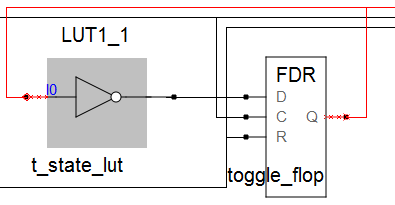
\includegraphics{t_state.png}



